\section{Method}
\label{sec:equi-vae}


This section presents our methodology. We first provide an overview of autoencoder models for latent generative modeling (\secref{sec:prelim}), focusing on the continuous case used in diffusion models. We then highlight the lack of equivariance in latent representations (\secref{sec:irregularity}) and introduce EQ-VAE to address it (\secref{sec:method-eqvae}).

\subsection{Preliminary: Continuous Autoencoders for Latent Generative Modeling}
\label{sec:prelim}

The first modeling stage consists of an autoencoder that compresses the pixel space into a continuous (\citet{rombach2022high}) or discrete (\citet{esser2021taming}) latent space. We focus here on the continuous case.
Given an input image $\mathbf{x} \in \mathbb{R}^{H \times W \times 3}$, an 
encoder $\mathcal{E}$ transforms the image into a compressed representation $\mathbf{z}= \mathcal{E(\mathbf{x})} \in \mathbb{R}^{\frac{H}{f} \times \frac{W}{f} \times c}$, where $f$ is the compression ratio and $c$ are the latent channels. Then a decoder $\mathcal{D}$ takes as input the latent representation and reconstructs the image $\hat{\mathbf{x}} = \mathcal{D}(\mathbf{z})$. For an input image $\mathbf{x}$ the training objective reads as follows:
\begin{align}
    \label{eq:ldm}
    \mathcal{L}_{\text{VAE}}(\mathbf{x}) = 
    % \underset{x\sim p(x)}{\mathbb{E}} 
    % \Big[ 
    \mathcal{L}_{rec}(\mathbf{x}, \mathbf{\hat{x}}) + \lambda_{gan} \mathcal{L}_{gan}(\mathbf{\hat{x}}) + 
    \lambda_{reg} \mathcal{L}_{reg}
    % \Big]
\end{align}
where $\mathcal{L}_{rec}$ consists of a pixel space reconstruction objective and a perceptual loss such LPIPS \cite{zhang2018unreasonable}, $\mathcal{L}_{gan}$ is a patch-based adversarial loss \cite{isola2017image}
%is an adversarial loss utilizing a patch-based discriminator \cite{isola2017image} 
and $\mathcal{L}_{reg}$ is usually a Kullback-Leibler regularization with a Gaussian prior \cite{kingma2014}.

\begin{figure}[t]
    \centering
    \setlength{\tabcolsep}{1.5pt}
    \begin{tabular}{cccc}
      \multirow{2}{*}{\small Input Image \textbf{x}}
      & \multicolumn{2}{c}{{\small \texttt{SD-VAE}}}
      & {\texttt{Ours}} \\
      \cmidrule(lr){2-3} \cmidrule(lr){4-4}
       
      & {\small$\mathcal{D} ( \mathcal{E}(\tau \circ \mathbf{x}))$}
      & {\small$\mathcal{D}(\tau \circ \mathcal{E}(\mathbf{x}))$}
      & {\small$\mathcal{D}(\tau \circ \mathcal{E}(\mathbf{x}))$} \\
      
      \vspace{-0.4cm} \\
      
     \includegraphics[width=0.225\linewidth]{fig/equi_latex_new/000051.png} 
      & \includegraphics[width=0.225\linewidth]{fig/equi_latex_new/51_before.JPEG} 
      & \includegraphics[width=0.225\linewidth]{fig/equi_latex_new/51_after.JPEG} 
      & \includegraphics[width=0.225\linewidth]{fig/equi_latex_new/51_ours.JPEG} \\
      
      \includegraphics[width=0.225\linewidth]{fig/equi_plots/images/00000046.JPEG} 
      & \includegraphics[width=0.225\linewidth]{fig/equi_plots/sd-vae/befre_s05/00000046.JPEG} 
      & \includegraphics[width=0.225\linewidth]{fig/equi_plots/sd-vae/s05/00000046.JPEG} 
      & \includegraphics[width=0.225\linewidth]{fig/equi_plots/ours/s05/00000046.JPEG} \\

    \end{tabular}
  \caption{
  \textbf{Latent Space Equivariance.} 
  Reconstructed images using \texttt{SD-VAE}~\cite{rombach2022high} and our \our when applying scaling transformation $\tau$, with factor $s=0.5$, to the input images $\mathcal{D}(\mathcal{E}(\tau \circ \mathbf{x}))$ versus directly to the latent representations $\mathcal{D}(\tau \circ \mathcal{E}(\mathbf{x}))$. Our approach preserves reconstruction quality under latent transformations, whereas \texttt{SD-VAE} exhibits significant degradation. See ~\autoref{fig:qualitative-equivariance-appendix} for additional examples.
  }
  \label{fig:qualitative-equivariance-main}
\end{figure}


% Define custom colors


\definecolor{SDVAE}{RGB}{0,128,128}          % Very Dark Blue
\definecolor{SDVAEOurs}{RGB}{0,100,100  }     % Bright Blue (unchanged)
\definecolor{SDXLVAE}{RGB}{44, 62, 80}        % Very Dark Orange
\definecolor{SDXLVAEOurs}{RGB}{255, 140, 0}   % Bright Orange (unchanged)





\begin{figure}[ht]
    \centering
    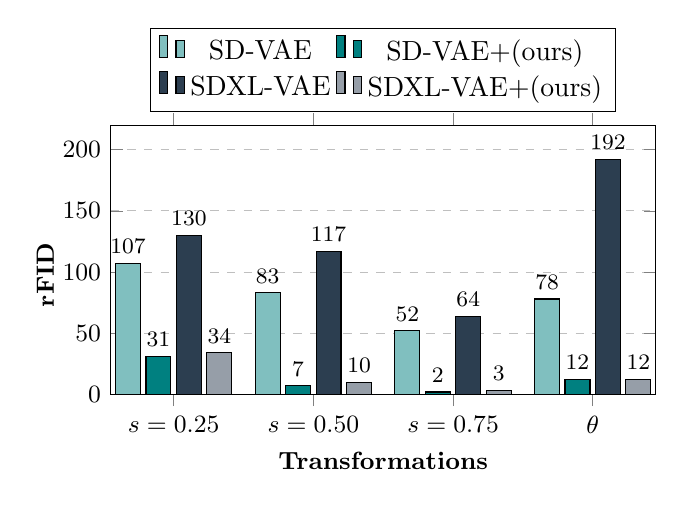
\begin{tikzpicture}
        \begin{axis}[
            ybar,
            width=8.5cm,
            height=5cm,
            bar width=9pt,
            ymin=0,
            ymax=220,
            ylabel={\Th{\textbf{rFID}}},
            y label style={
                at={(axis description cs:-0.12,0.6)}, % Adjust the position
                anchor=east                         % Align the label properly
            },
            xlabel={\textbf{Transformations}},
            symbolic x coords={$s=0.25$,$s=0.50$,$s=0.75$,$\theta$},
            xtick=data,
            ymajorgrids=true,
            grid style=dashed,
            enlarge x limits=0.15,
            legend style={
                at={(0.5,1.05)},
                anchor=south,
                legend columns=2,
            },
            nodes near coords,
            every node near coord/.append style={font=\footnotesize, anchor=south},
            label style={font=\small},
            ticklabel style={font=\small},
        ]
        
        % SD-VAE
        \addplot [
            fill=SDVAE!50, 
            draw=black, 
        ] coordinates {
            ($s=0.75$, 52)
            ($s=0.50$, 83)
            ($s=0.25$, 107)
            ($\theta$, 78)
        };
        
        % SD-VAE+(ours)
        \addplot [
            fill=SDVAE, 
            draw=black, 
        ] coordinates {
            ($s=0.75$, 2)
            ($s=0.50$, 7)
            ($s=0.25$, 31)
            ($\theta$, 12)
        };
        
        % SDXL-VAE
        \addplot [
            fill=SDXLVAE, 
            draw=black, 
        ] coordinates {
            ($s=0.75$, 64)
            ($s=0.50$, 117)
            ($s=0.25$, 130)
            ($\theta$, 192)
        };
        
        % SDXL-VAE+(ours)
        \addplot [
            fill=SDXLVAE!50, 
            draw=black, 
        ] coordinates {
            ($s=0.75$, 3)
            ($s=0.50$, 10)
            ($s=0.25$, 34)
            ($\theta$, 12)
        };
        
        \legend{SD-VAE, SD-VAE+(ours), SDXL-VAE, SDXL-VAE+(ours)}
        
        \end{axis}
    \end{tikzpicture}
    \caption{\textbf{Enhanced Reconstruction under Latent Transformations.} Reconstruction \Th{rFID} measured between $\tau \circ \mathbf{x}$ and $ \mathcal{D}(\tau \circ \mathcal{E}(\mathbf{x}))$ for various spatial transformations. We consider scaling transforms with factors $s = 0.75, 0.50, 0.25$ and also measure the average \Th{rFID}  over rotation angles $\theta = \frac{\pi}{2}, \pi, \frac{3\pi}{2}$. Results for \sdvae~\cite{rombach2022high} and \texttt{SDXL-VAE}~\cite{podell2024sdxl}, with and without \our. Our approach significantly reduces \Th{rFID} compared to baselines, improving image fidelity under latent transformations. For readability, we show $\floor{\Th{rFID}}$. }
    \label{fig:scales-rfig}
\end{figure}

\subsection{Lack of Equivarance under Spatial Tansformations}
\label{sec:irregularity}



Our work is motivated by a key observation: state-of-the-art autoencoders, such as \texttt{SD-VAE} \cite{rombach2022high}, produce latent representations 
$\mathcal{E}(\mathbf{x})$ that are not equivariant under basic spatial transformations like scaling and rotation. 

We formalize this as follows:

\noindent \textbf{Spatial Transformation} Let $\mathbf{x}(\mathbf{p}): \mathbb{R}^2 \rightarrow \mathbb{R}^c$ be an image (or latent representation) defined over 2D coordinates  \mbox{$\mathbf{p} = [u, v]^\top$}. 
A spatial transformation $\mathbf{\tau} \in \mathbb{R}^{2 \times 2}$ acts on the coordinates $p$ transforming $\mathbf{x}$ as follows:
\begin{equation} \label{eq:transformation}
\mathbf{x}_{\tau}(\mathbf{p}) =\mathbf{x}(\mathbf{\tau}^{-1} \mathbf{p})\text{,}
\end{equation}
denoted compactly for all $\mathbf{p}$ as $\tau \circ \mathbf{x}$.


\noindent \textbf{Equivariance} A latent representation $\mathcal{E}(\mathbf{x})$ is equivariant with a
transformation $\tau$ of the input image $\mathbf{x}$ if the transformation
can be transferred to the representation output: 
\begin{align}
    \label{eq:equivariace}
    \forall \mathbf{x} \in \mathcal{X}: \quad \mathcal{E}(\tau \circ \mathbf{x}) = \tau \circ \mathcal{E}(\mathbf{x})\text{.}
\end{align}

To test whether the latent representations of autoencoder models are equivariant under spatial transformations, we applied scaling and rotations $\tau$ directly to the latent code and evaluated the corresponding reconstructions. 
Specifically, we compare decoding transformed latent representations, $\mathcal{D}(\mathbf{\tau} \circ \mathcal{E}(\mathbf{x}))$, to decoding latents of transformed input images, $\mathcal{D}(\mathcal{E}(\mathbf{\tau} \circ \mathbf{x}))$. 
We present qualitative and quantitative results in \autoref{fig:qualitative-equivariance-main} and \autoref{fig:scales-rfig} respectively.

Our findings reveal a clear disparity: while autoencoders reconstruct images accurately when transformations are applied to the input (i.e., $\mathcal{D}(\mathcal{E}(\mathbf{\tau} \circ \mathbf{x}))$), applying transformations directly to the latent representation (i.e., $\mathcal{D}(\mathbf{\tau} \circ \mathcal{E}(\mathbf{x}))$) leads to significant degradation in reconstruction quality.

This limitation arises because (1) convolutional architectures commonly used in the autoencoders of latent generative models, such as \texttt{SD-VAE}, are not equivariant under arbitrary spatial transformations such as scaling and rotation, and (2) their standard training objectives (for example, reconstruction loss and KL divergence) do not explicitly or implicitly encourage equivariance. As a result, semantically similar inputs, such as an image $\mathbf{x}$ and its scaled counterpart $\mathbf{\tau} \circ \mathbf{x}$, are encoded into latent codes $\mathcal{E}(\mathbf{x})$ and $\mathcal{E}(\mathbf{\tau} \circ \mathbf{x})$ that are not related by the corresponding spatial transformation, i.e. $\mathcal{E}(\mathbf{\tau} \circ \mathbf{x}) \neq \mathbf{\tau} \circ \mathcal{E}(\mathbf{x})$, thus unnecessarily complicating the structure of the latent space.

\subsection{EQ-VAE: Regularization via equivariance constraints}
\label{sec:method-eqvae}

To address this limitation, we propose \texttt{EQ-VAE}, which regularizes the latent representations to promote equivariance under spatial transformations.
As seen in \autoref{fig:teaser} (left) this produces smoother latent representations, enabling more efficient learning.
% By simplifying the latent space, EQ-VAE reduces the burden on downstream generative models, enabling more efficient learning (see \autoref{fig:teaser}).

\noindent \textbf{Explicit Regularization.} 
A direct way to enforce equivariance is to include the equivariance constraint from \Equation{eq:equivariace} as a loss term during training:
\begin{equation}
    \label{eq:encoder_loss}
     \mathcal{L}_{\text{explicit}}(\mathbf{x}) = 
     % \underset{\substack{\tau \sim \mathcal{T}}}{\mathbb{E}}\big[ 
     \Vert \tau \circ \mathcal{E}(\mathbf{x}) - \mathcal{E}(\tau \circ  \mathbf{x}) \Vert_2^2 
     % \big]
     \text{,}
\end{equation}
where $\tau$ is sampled from a set of spatial transformations. However, minimizing this loss alone can lead to trivial solutions, such as collapsing the latent representation to a constant value $\mathcal{E}(\mathbf{x}) = \text{c}, \; \forall \mathbf{x}$, which we observe in our experiments (see \autoref{tab:losses}), making explicit regularization ineffective.


\noindent \textbf{Implicit Regularization.} 
To overcome this limitation of explicit regularization, we adopt an implicit approach. Inspired by the findings in \autoref{fig:qualitative-equivariance-main}, this approach aligns the reconstructions of transformed latent representations ($\mathcal{D}\big( \tau \circ \mathcal{E}(\mathbf{x}) \big)$) with the corresponding transformed inputs ($\tau \circ \mathbf{x}$ ). Specifically, we modify the original training objective of \Equation{eq:ldm} as follows:
\begin{align}
    \label{eq:ours_obj}
    \mathcal{L}_{\text{EQ-VAE}} (\mathbf{x}, {\color{DarkenedMagenta}{\tau}}) = 
     \mathcal{L}_{rec}& \Big({\color{DarkenedMagenta}{\text{$\mathbf{\tau} \circ$}}} \mathbf{x}, \mathcal{D}\big ({\color{DarkenedMagenta}{\text{$\mathbf{\tau} \circ$}}}\mathcal{E}(\mathbf{x}) \big) \Big) + \\
    \lambda_{gan} \mathcal{L}_{gan}& \Big( \mathcal{D}\big ({\color{DarkenedMagenta}{\text{$\mathbf{\tau} \circ$}}} \mathcal{E}(\mathbf{x}) \big) \Big) + \lambda_{reg} \mathcal{L}_{reg} \notag
    % \Big] 
\end{align}
where the changes compared to \Eq{eq:ldm} are highlighted in {\color{DarkenedMagenta}{color}}.
Notice that when $\tau$ is the identity transformation, this formulation reduces to the original objective in \Eq{eq:ldm}. By leveraging the rich supervision signal from both reconstruction and adversarial objectives, this approach implicitly encourages the encoder to produce equivariant latent representations while avoiding mode collapse (see \secref{sec:appenidx_exp_imp}).

\noindent \textbf{Transformation Design.} 
We focus on two types of spatial transformations: anisotropic scaling and rotations. These are parameterized as:
\begin{equation}
\mathbf{S}(s_x, s_y) =
\begin{bmatrix}
s_x  & 0 \\
0 &  s_y
\end{bmatrix}    
,\quad 
\mathbf{R}(\theta)=
\begin{bmatrix}
 \cos\theta & -\sin\theta \\
\sin\theta &   \cos\theta
\end{bmatrix}    
\end{equation}
The final transformation is the composition of scaling and rotation: $\tau = \mathbf{S}(s_x, s_y) \cdot \mathbf{R}(\theta)$.
We sample uniformly $0.25 < s_x, s_y < 1$, and $\theta \in ( \frac{\pi}{2},\pi, \frac{3\pi}{2})$. We consider these three rotation angles (multiples of 90$^{\circ}$) to avoid corner artifacts. For downsampling, we use bicubic interpolation. Empirically, we find \emph{scaling equivariance is more beneficial} for generation than rotation equivariance (see \autoref{tab:ablation-trans}).

To preserve the prior reconstruction capabilities of the autoencoder, we return to the standard objective (\Eq{eq:ldm}) by sampling the identity transform \(\tau = \mathbf{I}\) in \Eq{eq:ours_obj} with probability \(p_{\alpha}\). 
Our total objective can thus be written as:
\
\begin{align}
\mathcal{L}_{total}(\mathbf{x}) = 
\begin{cases}
    \mathcal{L}_{\text{VAE}}(\mathbf{x}) \qquad  & p <p_{\alpha}, \\
       % \underset{x\sim p(x)}{\mathbb{E}} 
    % \mathcal{L}_{\text{VAE}}(\mathbf{\tau_s} \circ \mathbf{x})  \qquad & p_{\alpha} \leq p < p_{\alpha}+ p_{\beta}, \\
   \mathcal{L}_{\text{EQ-VAE}}(\mathbf{x}, \tau) \qquad &   p \geq p_{\alpha} . \\
\end{cases}
\end{align}
where $p$ is  sampled uniformly from $[0, 1]$. This controls the strength of our regularization. By default we set $p_{\alpha}=0.5$  (we ablate regularization strength in \secref{sec:appendix_prior}).


We note that our approach enforces equivariance by applying transformations directly to the latent space, distinguishing it from methods relying on input data augmentation \cite{brehmer2024does}. 



\noindent \textbf{Extending EQ-VAE to Discrete Autoencoders.} So far, we described \our in the context of continuous autoencoders.
In discrete autoencoders e.g., \texttt{VQ-GAN}~\cite{esser2021taming}, the encoder outputs continuous features $\mathcal{E}(\mathbf{x})$ that are mapped to the nearest entry in a learned codebook, forming a discretized latent space via quantization. 
Adapting our method for discrete autoencoders, such as \texttt{VQ-GAN}, is straightforward. 
We employ our equivariance regularization loss as described in \secref{sec:method-eqvae} and apply the transformations $\tau$ on the latent features $\mathcal{E}(\mathbf{x})$ \emph{before} the quantization.
